\documentclass[12pt]{article}
\usepackage[margin=1in]{geometry}
\usepackage{sansmath} %Used for transpose T
\usepackage{amsmath} %Standard math library
\usepackage{mathtools}
\usepackage{enumitem} %Used for enumate lists
\usepackage{graphicx} %Used for image path
\usepackage[title]{appendix}
\usepackage{booktabs} %Better Table Horizontal Lines
\usepackage[numbered,framed]{matlab-prettifier}
\graphicspath{ {./images/} }%Sets image path
\let\ph\mlplaceholder % shorter macro
\usepackage{subcaption} %MAC Compatibility
\captionsetup{compatibility=false}
\lstMakeShortInline"
\lstset{
  style              = Matlab-editor,
  basicstyle         = \mlttfamily,
  escapechar         = ',
  mlshowsectionrules = true,
}
\title{Sudoku Solver by Linear Programming}
\author{Thomas M. Gira}
\date{May 3rd, 2022}
\begin{document}
\maketitle
\begin{abstract}
This paper outlines and solves the problem of solving a sudoku grid using methods of linear programming.
Uses of this project extends to many applications especially those constained to integer values such as determining workforces. 
This project compares methods used with linear programming to optimized methods of brute force. Ultimatesly and not
suprisingly linear programming wins in most cases with compute times in micro-seconds while brute force is in the hours.
Interestingly linear programming does not find a deterministic solution and on complicated boards it may fail to converge.
\end{abstract}
\pagenumbering{gobble}
\section{Introduction}
The goal of this project is to solve sudoku using linear programming, initially starting with a 4x4 grid before
moving into a more typical 9x9 grid. It uses standard form linear programming with only equality constraints. This
allows for solving using traditional methods, in this this case the "linprog" feature of MATlab. 
\begin{figure}
\centering
\begin{subfigure}{.5\textwidth}
  \centering
  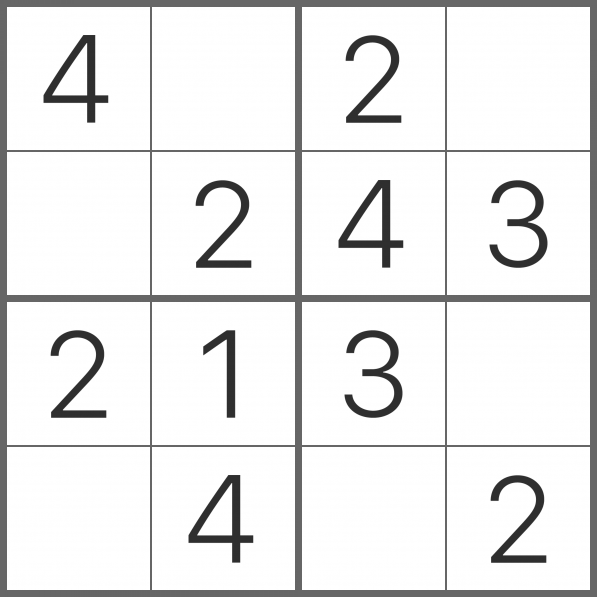
\includegraphics[width=.4\linewidth]{4x4}
  \caption{Smaller 4x4 Grid}
  \label{fig:sub1}
\end{subfigure}%
\begin{subfigure}{.5\textwidth}
  \centering
  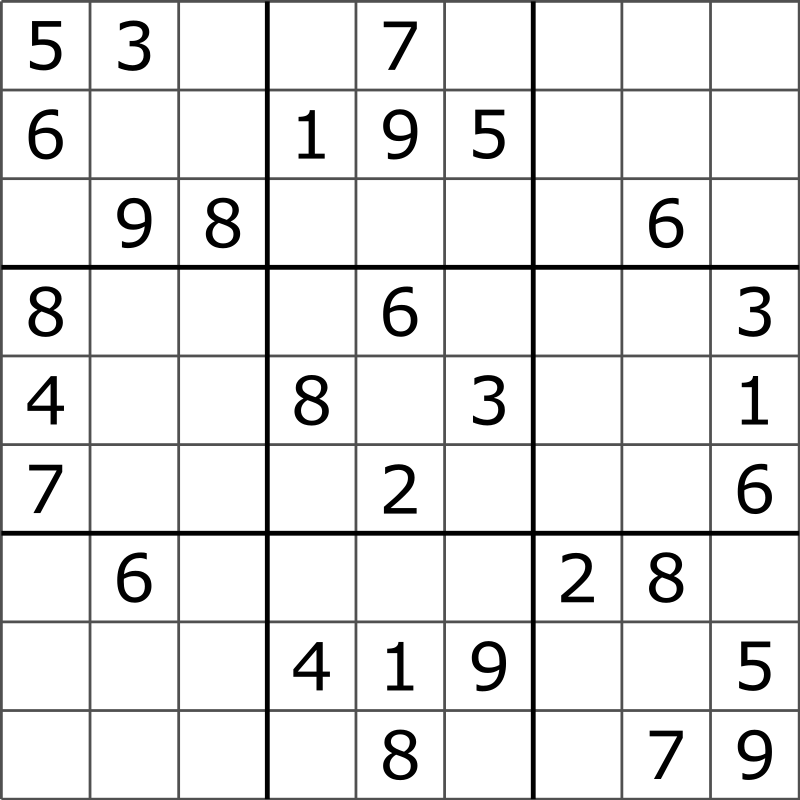
\includegraphics[width=.4\linewidth]{9x9}
  \caption{Traditional 9x9 Grid}
  \label{fig:sub2}
\end{subfigure}
\caption{Example Sudoku Grids}
\label{fig:sud}
\end{figure}
This problem utilized the two grid sizes shown in figure \ref{fig:sud} for two distinct purposes. First when developing
the code necessary to solve this problem it was faster to troubleshoot on a 4x4 grid instead of a 9x9 grid. Additionally
when solving for a 4x4 grid using brute force the possibile solutions are cut down drastically reducing speeds by exponential
magnitudes.
\\

\section{Least Norm}
To solve this problem, it needs to be understood that it is an integer problem and least norm cannot be used to solve
integer problems. So, in order to solve an integer problem using least norm we need to do a lot of manipulation. First
we consider each location of a number to be a cell. For a grid with nxn cells each cell can be a number ranging from 1-n.
There are $n^2$ possible cells each of which each have n possible values. In order to ensure that they will be integer values
we create n variables for each cell which represent if that cell is occupied by that value or not. This still doesnt
solve the issue of least norm completely. In order to make it so that the occupancy of a number is as close to a boolean value
as possible we first limit it to being between 1 and zero and then use a 1 norm to have as many zeros as possible. Additionally
techniques were used to create uniquness and restain the number of values in a cell. Even with these constraints the solution
is still not deterministic and in some uniuqe cases the algorithm will fail.

\section{Variables}
In order to solve this problem it was essential to create the necessary constraints, which often have strange configurations.
To understand these constriants it is important to first look at what each variable is, in our case we will use the example of a 4x4
grid however these matrices can be expanded to a 9x9 grid as well. Looking at the grid:
$$
\begin{bmatrix}
x\_\{0\}  & x\_\{1\}  & x\_\{2\}  & x\_\{3\}  \\
x\_\{4\}  & x\_\{5\}  & x\_\{6\}  & x\_\{7\}  \\
x\_\{8\}  & x\_\{9\}  & x\_\{10\} & x\_\{11\} \\
x\_\{12\} & x\_\{13\} & x\_\{14\} & x\_\{15\}
\end{bmatrix}
$$
we can see that there are 16 variables however there needs to be 4 variables for each cell not just a single, there fore we create the grid:
$$
\begin{bmatrix}
x\_\{0\},...,x\_\{3\}   & x\_\{4\},...,x\_\{7\}   & x\_\{8\},...,x\_\{11\}  & x\_\{12\},...,x\_\{15\} \\
x\_\{16\},...,x\_\{19\} & x\_\{20\},...,x\_\{23\} & x\_\{24\},...,x\_\{27\} & x\_\{28\},...,x\_\{31\} \\
x\_\{32\},...,x\_\{35\} & x\_\{36\},...,x\_\{39\} & x\_\{40\},...,x\_\{43\} & x\_\{44\},...,x\_\{47\} \\
x\_\{48\},...,x\_\{51\} & x\_\{52\},...,x\_\{55\} & x\_\{56\},...,x\_\{59\} & x\_\{60\},...,x\_\{63\}
\end{bmatrix}
$$
Now we have the 64 variables that we expect, ranging from 1 to 0 representative of whether a cell is filled with that value or not.
We can then mimize the one norm of these variables in order to create as many zeros as possible and attempt to create a binary/
integer problem.

This can also be expanded to problems with a square grid whose length and width are a square number. In the general case of an 9x9 grid
there will be $n^3$ total variables.

\section{Constraints}
Using the afermentioned variables we can begin to create constraints to define the problem correctly. For my solution I 
utilized only equality constraints. To visualize these constraints we continue to use a 4x4 grid example.

The first constraint implemented is the row constraint. This constraint ensures that the sum of each row is equal to
the sum of 1+2+...+n where n is the grid size. With this constraint we attempt to esnure that each row has the correct numbers in it.
To create this constraint we first create the vector:
$$
\hat{nr} =
\begin{bmatrix}
1 & 2 & \hdots & n
\end{bmatrix}
$$
from that we create the matrix:
$$
\hat{A} =
\begin{bsmallmatrix}
\hat{nr} & \hat{nr} & \hat{nr} & \hat{nr} & \hat{0} & \hat{0} & \hat{0} & \hat{0} & \hat{0} & \hat{0} & \hat{0} & \hat{0} & \hat{0} & \hat{0} & \hat{0} & \hat{0} \\
\hat{0} & \hat{0} & \hat{0} & \hat{0} & \hat{nr} & \hat{nr} & \hat{nr} & \hat{nr} & \hat{0} & \hat{0} & \hat{0} & \hat{0} & \hat{0} & \hat{0} & \hat{0} & \hat{0} \\
\hat{0} & \hat{0} & \hat{0} & \hat{0} & \hat{0} & \hat{0} & \hat{0} & \hat{0} & \hat{nr} & \hat{nr} & \hat{nr} & \hat{nr} & \hat{0} & \hat{0} & \hat{0} & \hat{0} \\
\hat{0} & \hat{0} & \hat{0} & \hat{0} & \hat{0} & \hat{0} & \hat{0} & \hat{0} & \hat{0} & \hat{0} & \hat{0} & \hat{0} & \hat{nr} & \hat{nr} & \hat{nr} & \hat{nr} \\
\end{bsmallmatrix}
$$
The next constraint that we solve is the column constrain, this has a similar format to the row constraint, using the same
$\hat{nr}$ vector. It however, results in the matrix:
$$
\hat{A} =
\begin{bsmallmatrix}
\hat{nr} & \hat{0} & \hat{0} & \hat{0} & \hat{nr} & \hat{0} & \hat{0} & \hat{0} & \hat{nr} & \hat{0} & \hat{0} & \hat{0} & \hat{nr} & \hat{0} & \hat{0} & \hat{0} \\
\hat{0} & \hat{nr} & \hat{0} & \hat{0} & \hat{0} & \hat{nr} & \hat{0} & \hat{0} & \hat{0} & \hat{nr} & \hat{0} & \hat{0} & \hat{0} & \hat{nr} & \hat{0} & \hat{0} \\
\hat{0} & \hat{0} & \hat{nr} & \hat{0} & \hat{0} & \hat{0} & \hat{nr} & \hat{0} & \hat{0} & \hat{0} & \hat{nr} & \hat{0} & \hat{0} & \hat{0} & \hat{nr} & \hat{0} \\
\hat{0} & \hat{0} & \hat{0} & \hat{nr} & \hat{0} & \hat{0} & \hat{0} & \hat{nr} & \hat{0} & \hat{0} & \hat{0} & \hat{nr} & \hat{0} & \hat{0} & \hat{0} & \hat{nr} \\
\end{bsmallmatrix}
$$
The last constraint of this type is the box constraint of form:
$$
\hat{A} =
\begin{bsmallmatrix}
\hat{nr} & \hat{nr} & \hat{0} & \hat{0} & \hat{nr} & \hat{nr} & \hat{0} & \hat{0} & \hat{0} & \hat{0} & \hat{0} & \hat{0} & \hat{0} & \hat{0} & \hat{0} & \hat{0} \\
\hat{0} & \hat{0} & \hat{nr} & \hat{nr} & \hat{0} & \hat{0} & \hat{nr} & \hat{nr} & \hat{0} & \hat{0} & \hat{0} & \hat{0} & \hat{0} & \hat{0} & \hat{0} & \hat{0} \\
\hat{0} & \hat{0} & \hat{0} & \hat{0} & \hat{0} & \hat{0} & \hat{0} & \hat{0} & \hat{nr} & \hat{nr} & \hat{0} & \hat{0} & \hat{nr} & \hat{nr} & \hat{0} & \hat{0} \\
\hat{0} & \hat{0} & \hat{0} & \hat{0} & \hat{0} & \hat{0} & \hat{0} & \hat{0} & \hat{0} & \hat{0} & \hat{nr} & \hat{nr} & \hat{0} & \hat{0} & \hat{nr} & \hat{nr} \\
\end{bsmallmatrix}
$$
Each of these matrices has the same b matrix equal to the sum of valid numbers:
$$
b = 
\begin{bmatrix}
10 & 10 & 10 & 10
\end{bmatrix},
$$

After implementing these contraints you may find that you rend up with a solution however there are multiple empty cells and cells with partial values instead of a
confident one. One step to solve this is to add in a new constraint that ensures that there is only one of each possible number in every row, column and box.
For rows this is accomplished using the matrix:
$$
\hat{A} =
\begin{bsmallmatrix}
\hat{I_n} & \hat{I_n} & \hat{I_n} & \hat{I_n} & \hat{0} & \hat{0} & \hat{0} & \hat{0} & \hat{0} & \hat{0} & \hat{0} & \hat{0} & \hat{0} & \hat{0} & \hat{0} & \hat{0} \\
\hat{0} & \hat{0} & \hat{0} & \hat{0} & \hat{I_n} & \hat{I_n} & \hat{I_n} & \hat{I_n} & \hat{0} & \hat{0} & \hat{0} & \hat{0} & \hat{0} & \hat{0} & \hat{0} & \hat{0} \\
\hat{0} & \hat{0} & \hat{0} & \hat{0} & \hat{0} & \hat{0} & \hat{0} & \hat{0} & \hat{I_n} & \hat{I_n} & \hat{I_n} & \hat{I_n} & \hat{0} & \hat{0} & \hat{0} & \hat{0} \\
\hat{0} & \hat{0} & \hat{0} & \hat{0} & \hat{0} & \hat{0} & \hat{0} & \hat{0} & \hat{0} & \hat{0} & \hat{0} & \hat{0} & \hat{I_n} & \hat{I_n} & \hat{I_n} & \hat{I_n} \\
\end{bsmallmatrix}
$$
The next constraint that we solve is the column constrain, this has a similar format to the row constraint. However, results in the matrix:
$$
\hat{A} =
\begin{bsmallmatrix}
\hat{I_n} & \hat{0} & \hat{0} & \hat{0} & \hat{I_n} & \hat{0} & \hat{0} & \hat{0} & \hat{I_n} & \hat{0} & \hat{0} & \hat{0} & \hat{I_n} & \hat{0} & \hat{0} & \hat{0} \\
\hat{0} & \hat{I_n} & \hat{0} & \hat{0} & \hat{0} & \hat{I_n} & \hat{0} & \hat{0} & \hat{0} & \hat{I_n} & \hat{0} & \hat{0} & \hat{0} & \hat{I_n} & \hat{0} & \hat{0} \\
\hat{0} & \hat{0} & \hat{I_n} & \hat{0} & \hat{0} & \hat{0} & \hat{I_n} & \hat{0} & \hat{0} & \hat{0} & \hat{I_n} & \hat{0} & \hat{0} & \hat{0} & \hat{I_n} & \hat{0} \\
\hat{0} & \hat{0} & \hat{0} & \hat{I_n} & \hat{0} & \hat{0} & \hat{0} & \hat{I_n} & \hat{0} & \hat{0} & \hat{0} & \hat{I_n} & \hat{0} & \hat{0} & \hat{0} & \hat{I_n} \\
\end{bsmallmatrix}
$$
The last constraint of this type is the box constraint of form:
$$
\hat{A} =
\begin{bsmallmatrix}
\hat{I_n} & \hat{I_n} & \hat{0} & \hat{0} & \hat{I_n} & \hat{I_n} & \hat{0} & \hat{0} & \hat{0} & \hat{0} & \hat{0} & \hat{0} & \hat{0} & \hat{0} & \hat{0} & \hat{0} \\
\hat{0} & \hat{0} & \hat{I_n} & \hat{I_n} & \hat{0} & \hat{0} & \hat{I_n} & \hat{I_n} & \hat{0} & \hat{0} & \hat{0} & \hat{0} & \hat{0} & \hat{0} & \hat{0} & \hat{0} \\
\hat{0} & \hat{0} & \hat{0} & \hat{0} & \hat{0} & \hat{0} & \hat{0} & \hat{0} & \hat{I_n} & \hat{I_n} & \hat{0} & \hat{0} & \hat{I_n} & \hat{I_n} & \hat{0} & \hat{0} \\
\hat{0} & \hat{0} & \hat{0} & \hat{0} & \hat{0} & \hat{0} & \hat{0} & \hat{0} & \hat{0} & \hat{0} & \hat{I_n} & \hat{I_n} & \hat{0} & \hat{0} & \hat{I_n} & \hat{I_n} \\
\end{bsmallmatrix}
$$
Each of these matrices has the same b matrix equal to the number of cells in a row, column or box:
$$
b = 
\begin{bsmallmatrix}
4 & 4 & 4 & 4 & 4 & 4 & 4 & 4 & 4 & 4 & 4 & 4 & 4 & 4 & 4 & 4 \\ 
\end{bsmallmatrix}'
$$

An additional constraint is to set the sum of variables in each cell equal to one to prevent empty cells or overfilled cells. The last and final constraint is to convert
the given board into a form fitting the variable scheme used and then set the any filled variable equal to zero.

\section{Rust}
I'm not actually sure if we were supposed to do an extra step for the grad level but I though it would be fun to try and brute force this project. Now obviously there
are a large number of possibilites when trying to brute force the solution so I did what any sane person would do and learned the most optimized programming language
to do it in. Rust is a c++ like programming language that performs intense optimization and creates code that is universal and memory safe. So, I though it would be a
lanugage to learn and experiment in. To start this I made a class that contains the game. It saves the current board and performs logic to check rows, colimns and boxes 
all expandable to n dimensions. I then needed to iterate through possibilities. 

My initial attempt had a for loop of from 1 to $n^t$ where $t$ is the number of empty cells and 
$n$ is the number of possible values. I then dereferenced the numbers mod $n$. Essentially I put the number into binary but instead of being 0 or 1 it was the 
numbers $0,1,\hdots,n-1$. This worked well enough and I was able to brute force the solution for a 4x4 grid in 19 seconds. Then I tried a 9x9 and it broke. Since of the way
I am dereferencing numbers you have to have absolute solution using an integer and cant use the precision that using a float will do. This means that with all of the potential
possibilities of a 9x9 grid you create a solution set that is so large it cant even be represented by a 128 bit unsigned integer. Since rust doesnt have any native integers
larger than 128 bits I decided I needed a new approach. This time I would use another class. 

I created a class that would increment through each possible arrangment of numbers without the issue of integer overflow. Running on a 4x4 we were now down to 13 seconds. 
However, with some quick napkin math it turns out it will take $10^{40}$ years to solve.As patient as I am I decided it was time for attept number 3. 
This time I would actually try and solve the problem (I didnt actually). 

I decided to preprocess the information before performing the brute force search and I elimated all possibilities that are impossible from the inital given solution. 
For a 4x4 grid, at least my test case, this solved in 0.000264 seconds, reducing the solution size to a single solution. So now I'm thinking this might actually possible 
so I plug in a 9x9 grid. However, there are 4,294,967,295 possible solutions, and with my back of the hand math; 
this will take 12 hours to solve. Says something for linear algebra.
 
In case you want to try out this script you can run it using ./main when in my "RUST" directory. Currently its compiled for unix so it should run without any dependencies.
You may have to install a rust compiler but honestly its not that interesting to watch run.
\section{Results}
Looking at the results of this project we see that it is possible to solve many simple cases of a sudoku grid however, expanding to more complex examples it will sometimes fail.
It is clearly demonstrated that solving using methods of linear programming is the quickest solution and requires far less problem setup and thinking than creating 
a brute for or more algorithmic solution.

\section{Conclusion}
This was a fun way to wrap up the class. I was excited to work o nthe project and it was one that reamined interesting through solving and debugging code.
Learning rust was an interesting experience and only time will tell if it becomes useful or not. I am interested in creating a algorithmic solution to solve it
however, the solution would have to be recursive and thats a bit complicated in rust. I think it would be interestinng to solve it where only game constraints bind the problem
not creating logic to solve it how a human would. This give more opportunity for the computer to optimize the solution, I think. This whole area is still a little above my paygrade.
\clearpage
\newpage
\appendix
\begin{Huge} Appendix \end{Huge}
\section{main.m}
\begin{verbatim}
%% Maintanence
clc
clear
close all

%% Project Setup
 s40 = [0 0 0 0;
        0 0 0 0;
        0 0 0 0;
        0 0 0 0];
 s41 = [0 1 0 0;
        3 0 0 1;
        4 0 0 2;
        0 0 4 0];
 s91 = [5 3 0 0 7 0 0 0 0;
        6 0 0 1 9 5 0 0 0;
        0 9 8 0 0 0 0 6 0;
        8 0 0 0 6 0 0 0 3;
        4 0 0 8 0 3 0 0 1;
        7 0 0 0 2 0 0 0 6;
        0 6 0 0 0 0 2 8 0;
        0 0 0 4 1 9 0 0 5;
        0 0 0 0 8 0 0 7 9];
 S41 = solve_sudoku(s41);
 S91 = solve_sudoku(s91);
 %% Funtions
 function solved = solve_sudoku(board)
    [m,~] = size(board);
    flat_board = reshape(board',1,m^2);
    print_sudoku(board)
    [Aeq,beq] = equality(m,flat_board);
    c = cost(m);
    x = linprog(c,[],[],Aeq,beq,zeros(m^3,1),ones(m^3,1));
    solved = convert_sudoku(x);
    print_sudoku(solved)
 end
 function [a,b] = equality(m,flat_board)
    [a_row,b_row] = row(m);
    [a_col,b_col] = col(m);
    [a_box,b_box] = box(m);
    [a_unique_row,b_unique_row] = unique_row(m);
    [a_unique_col,b_unique_col] = unique_col(m);
    [a_unique_box,b_unique_box] = unique_box(m);
    [a_single,b_single] = single_digit(m);
    [a_given,b_given] = given(m,flat_board);
    a = [a_row;a_col;a_box;a_given;a_single;a_unique_row;a_unique_col;a_unique_box];
    b = [b_row;b_col;b_box;b_given;b_single;b_unique_row;b_unique_col;b_unique_box];
 end
 function [a,b] = given(m,flat_board)
    a = zeros(m^3);
    b = zeros(m^3,1);
    for i = 1:m^2
        if flat_board(i) ~=0
            index = (i-1)*m + flat_board(i);
            a(index,index) = 1;
            b((i-1)*m+flat_board(i)) = 1;
        end
    end
 end
 function [a,b] = row(m)
    a = zeros(m,m^3);
    num_range = 1:m;
    nums = zeros(1,m^2);
    for i = 1:m
        nums(m*(i-1)+1:m*(i-1)+m) = num_range;
    end
    sum = m*(m + 1)/2;
    for i = 1:m
        a(i,:) = [zeros(1,(i-1)*m^2) nums zeros(1,m^2*(m-i))];
    end
    b = ones(m,1)*sum;
    %a = [a zeros(m,m^3)]; %Account for one norm
 end
 function [a, b] = col(m)
    a = zeros(m,m^3);
    num_range = 1:m;
    sum = m*(m + 1)/2;
    for i = 1:m
        i_offset = m*(i-1);
        for j = 1:m
            j_offset = m^2*(j-1);
            a(i,j_offset+1+i_offset:j_offset+m+i_offset) = num_range;
        end
    end
    b = ones(m,1)*sum;
    %a = [a zeros(m,m^3)]; %Account for one norm
 end
 function [a,b] = box(m)
    a = zeros(m,m^3);
    num_range = 1:m;
    sum = m*(m + 1)/2;
    n = sqrt(m);
    for i = 1:n
        i_offset = n*m^2*(i-1);
        for j = 1:n
            j_offset = n*m*(j-1);
            for k = 1:n
                k_offset = m^2*(k-1);
                for l = 1:n
                    l_offset = m*(l-1);
                    offset = i_offset + j_offset + k_offset + l_offset;
                    a(n*(i-1)+j,offset+1:offset+m) = num_range;
                end
            end
        end
    end
    b = ones(m,1)*sum;
    %a = [a zeros(m,m^3)]; %Account for one norm
 end
 function c = cost(m)
    c = ones(1,m^3);
 end
 function [a,b] = unique_row(m)
    a = zeros(m^2,m^3);
    for i = 1:m
        i_index = (i-1)*m^2;
        for j = 1:m
            j_index = m*(j-1);
            index = i_index + j_index;
            a(m*(i-1)+1:m*(i-1)+m,index+1:index+m) = eye(m);
        end
    end
    b = ones(m^2,1);
    %a = [a zeros(m,m^3)]; %Account for one norm
 end
 function [a,b] = unique_col(m)
    a = zeros(m^2,m^3);
    for i = 1:m
        nums = [zeros(m,(i-1)*m) eye(m) zeros(m,(m-i)*m)];
        i_index = (i-1)*m;
        for j = 1:m
            j_index = (j-1)*m^2;
            a(i_index+1:i_index+m,j_index+1:j_index+m^2) = nums;
        end
    end
    b = ones(m^2,1);
    %a = [a zeros(m,m^3)]; %Account for one norm
 end
 function [a,b] = unique_box(m)
    a = zeros(m^2,m^3);
    n = sqrt(m);
    for i = 1:n
        i_offset = n*m^2*(i-1); %Row * Cell
        for j = 1:n
            j_offset = n*m*(j-1); %Col * Cell
            index = (i-1)*m*n+(j-1)*m;
            for k = 1:n
                k_offset = m^2*(k-1); %Row
                for l = 1:n
                    l_offset = m*(l-1); %Cell
                    offset = i_offset + j_offset + k_offset + l_offset;
                    a(index+1:index+m,offset+1:offset+m) = eye(m);
                end
            end
        end
    end
    b = ones(m^2,1);
    %a = [a zeros(m,m^3)]; %Account for one norm
 end
 function print_sudoku(board)
    [m,~] = size(board);
    num_cells = sqrt(m);
    fprintf('\n') %Start on new row
    for i = 1:m %Loop through rows
        for j = 1:m
            fprintf('%i', board(i,j));
            if (mod(j,num_cells) == 0) && (j ~=0) && (j~=m)
                fprintf('|')
            end
        end
        fprintf('\n')
        if (mod(i,num_cells) == 0) && (i ~=0) && (i~= m)
            for k = 1:(m+num_cells-1)
                fprintf('-');
            end
            fprintf('\n')
        end
    end
    
 end
 function [a,b] = single_digit(m)
    nums = ones(1,m);
    a = zeros(m^2,m^3);
    b = ones(m^2,1);
    for i = 1:m^2
        a(i,(i-1)*m+1:(i-1)*m+m) = nums;
    end
 end
 function solved = convert_sudoku(x)
    m = uint64((length(x))^(1/3));
    sudoku = zeros(m^2,1);
    vals = 1:m;
    for i = 1:m^2
        for j = 1:m
            if x((i-1)*m+j) > 0
                sudoku(i) = vals(j);
            end
        end
    end
    solved = reshape(sudoku,m,m)';
 end
\end{verbatim}
\clearpage
\section{main.rs}
\begin{verbatim}
mod game;
mod prediction;
mod reduction;
use std::time::Instant;

fn main()
{
    let list1 = vec![0, 1, 0, 0, 
                    3, 0, 0, 1, 
                    4, 0, 0, 2, 
                    0, 0, 4, 0];
    let _list2 = vec![5, 3, 0, 0, 7, 0, 0, 0, 0, 
                    6, 0, 0, 1, 9, 5, 0, 0, 0,
                    0, 9, 8, 0, 0, 0, 0, 6, 0,
                    8, 0, 0, 0, 6, 0, 0, 0, 3,
                    4, 0, 0, 8, 0, 3, 0, 0, 1,
                    7, 0, 0, 0, 2, 0, 0, 0, 6,
                    0, 6, 0, 0, 0, 0, 2, 8, 0,
                    0, 0, 0, 4, 1, 9, 0, 0, 5,
                    0, 0, 0, 0, 8, 0, 0, 7, 9,];
    
    
    let now = Instant::now();
    brutus(&list1,4);
    let elapsed_time = now.elapsed();
    println!("Running brutus() took {:.6} seconds.", elapsed_time.as_micros() as f64/1000000.0);
    
    let now = Instant::now();
    big_brother(&list1,4);
    let elapsed_time = now.elapsed();
    println!("Running big_brother() took {:.6} seconds.", elapsed_time.as_micros() as f64/1000000.0);
    
    let now = Instant::now();
    doku(&list1,4);
    let elapsed_time = now.elapsed();
    println!("Running doku() took {:.6} seconds.", elapsed_time.as_micros() as f64/1000000.0);
    
    let now = Instant::now();
    doku(&_list2,9);
    let elapsed_time = now.elapsed();
    println!("Running doku() took {:.6} seconds.", elapsed_time.as_micros() as f64/1000000.0);
} 

fn brutus(list: &Vec<u32>, game_size: u128){
    println!("");
    println!("");
    println!("Running Brutus on a {}x{} Grid", game_size, game_size);
    println!("");
    println!("");
    let mut i: u128 = 0;
    let num_to_solve = list.to_vec().iter().filter(|&n| *n == 0).count() as u128;
    println!("num_to_solve: {}", num_to_solve);
    let max_val:u128 = game_size.pow((num_to_solve) as u32) -1;
    println!("max_value: {}", max_val);

    let mut last_percent: f64 = 0.0;
    let mut curr_percent: f64;

    while i < max_val {
        curr_percent = (i as f64)/(max_val as f64)*100.0;
        if (curr_percent/5.0).floor() > last_percent{
            println!("{:.0}% Complete",curr_percent);
            last_percent = (curr_percent/5.0).floor();
        }
        let mut p = game::Sudoku::new(list.to_vec(),game_size as u32);
        let combinations = deref(i as u128, game_size as u128,1);
        //println!("Combinations: {:?}", combinations);
        let placements = merge(list.to_vec(),combinations);
        // println!("Placements: {:?}", placements);
        i = i+1;
        for k in 0..game_size.pow(2){
            let position = deref(k as u128,4,0);
            
            if !p.add_number(position[1] as u32,position[0] as u32,placements[k as usize]){
                break;
            }
        }
        if p.is_solved(){
            p.print_board();
            return;
        }
    }
}

fn big_brother(list: &Vec<u32>, game_size: u32){
    println!("");
    println!("");
    println!("Running Big Brother on a {}x{} Grid", game_size, game_size);
    println!("");
    let mut given: Vec<(u32,u32)> = vec![];
    let num_to_solve = list.to_vec().iter().filter(|&n| *n == 0).count() as u32;
    let max_val:f64 = (game_size as f64).powf((num_to_solve) as f64) -1.0;
    println!("num_to_solve: {}", num_to_solve);
    println!("max_value: {}", max_val);
    for i in 0..game_size*game_size{
        if list[i as usize] != 0{
            given.push((i,list[i as usize]));
        }
    }
    let mut q = prediction::Prediction::new(given, game_size);
    q.initialize();
    let mut last_percent: f64 = 0.0;
    let mut i: f64 = 0.0;
    let mut curr_percent: f64;
    loop {
        i = i+1.0;
        curr_percent = (i as f64)/(max_val as f64)*100.0;
        if (curr_percent/5.0).floor() > last_percent{
            println!("{:.0}% Complete Index: {}",curr_percent,i);
            last_percent = (curr_percent/5.0).floor();
        }
        let mut p = game::Sudoku::new(list.to_vec(), game_size);
        if ! q.iter_prediction() {
            println!("Reached maximum iterations without as solution");
            return;
        }
        let prediction = q.get_prediction().to_vec();
        for k in 0..game_size.pow(2){
            let position = deref(k as u128,4,0);
            
            if !p.add_number(position[1] as u32, position[0] as u32, prediction[k as usize]){
                break;
            }
        }
        if p.is_solved(){
            p.print_board();
            return;
        }
    }
}

fn doku(list: &Vec<u32>, game_size: u32){
    println!("");
    println!("");
    println!("Running Doku on a {}x{} Grid", game_size, game_size);
    println!("");
    println!("");
    let mut given: Vec<(u32,u32)> = vec![];
    for i in 0..game_size*game_size{
        if list[i as usize] != 0{
            given.push((i,list[i as usize]));
        }
    }
   let mut q = reduction::Reduction::new(given,list.to_vec(), game_size as u32);
   q.initialize();
   let num_elements = q.get_num_possibilities();
   println!("Number of Possibilites: {}", num_elements);

   for i in 0..num_elements{
       q.iter_prediction();
       let prediction = q.get_prediction();
       let mut p = game::Sudoku::new(list.to_vec(), game_size);
        for k in 0..game_size.pow(2){
            let position = deref(k as u128,4,0);
            
            if !p.add_number(position[1] as u32, position[0] as u32, prediction[k as usize]){
                break;
            }
        }
        if p.is_solved(){
            p.print_board();
            return;
        }
    }
}

fn merge(mut base: Vec<u32>, mut supp: Vec<u32>) -> Vec<u32>{
    let length: u32 = base.len() as u32;
    supp.reverse();
    for i in 0..length{
        if base[i as usize] == 0{
            base[i as usize] = match supp.pop() {
                Some(top) => top,
                None => 0
            };
        }
    }
    return base
}

fn deref(reference: u128, base:u128, offset:u128) -> Vec<u32> {
    let mut indices: Vec<u32> = Vec::new();
    let mut temp: u128 = reference;
    for i in 1..base*base+1 {
        let div: u128 = base.pow((base*base-i)as u32);
        let sub: u128 = temp/div;
        indices.insert(0,(sub + offset) as u32);
        temp = temp - sub*div;
    }
    return indices;
}
\end{verbatim}
\clearpage
\section{game.rs}
\begin{verbatim}
pub struct Sudoku{
    board:Vec<u32> ,
    size: u32,
    grid_size: u32
}

impl Sudoku {

    pub fn new(initial_board: Vec<u32>, game_size: u32) -> Sudoku {
        Sudoku {
            board: initial_board,
            size: game_size,
            grid_size: f64::sqrt(game_size as f64) as u32
        }
    }

    pub fn print_board(&self){
        println!("");
        for i in 0..self.size {
            for j in 0..self.size {
                let index: u32 = i* self.size + j;
                print!("{}",self.board[index as usize]);
                if j % self.grid_size == 1 && j != self.size -1{
                    print!("|");
                }
            }
            if i % self.grid_size == 1 && i != self.size -1{
                println!("");
                for _ in 0..self.size+ self.grid_size -1{
                    print!("-");
                }
            }
            println!("");
        }
        println!("");
    }

    pub fn add_number(&mut self, y: u32, x: u32, number: u32) -> bool{
        let index: usize = (y*self.size + x) as usize;
        if number < 1 || number > self.size{
            //println!("Error: Invalid Number");
            return false;
        }
        if self.board[index] != 0 {
            // println!("Error: Index {} already filled",index);
            if self.board[index] == number{
                // println!("ASDSD");
                return true;
            }
            return false;
        }
        let mut temp_board: Vec<u32> = Vec::new();
        for i in 0..self.size*self.size{
            temp_board.push(self.board[i as usize]);
        }
        temp_board[index] = number;
        if self.check_valid_placement(temp_board.to_vec()){
            self.board = temp_board.to_vec();
            return true;
        }
        return false;
    }

    fn check_valid_placement(&self,board: Vec<u32>) -> bool{
        if ! self.check_valid_box(board.to_vec()){
            return false;
        }
        if ! self.check_valid_row(board.to_vec()){
            return false;
        }
        if ! self.check_valid_col(board.to_vec()){
            return false;
        }
        return true;
    }

    fn check_valid_row(&self,board: Vec<u32>) -> bool{
        let mut valid_numbers: Vec<u32> = Vec::new();
        let mut index: u32;
        let mut value: u32;
        for i in 0..self.size{
            for k in 0..self.size {
                valid_numbers.push(k+1 as u32);
            }
            for j in 0.. self.size{
                index = i*self.size + j;
                value = board[index as usize];
                if value > 0 {
                    if valid_numbers[(value -1) as usize] == 0{
                        //println!("Error: Invalid Row");
                        return false;
                    } else {
                        valid_numbers[(value -1) as usize] = 0;
                    }
                }
            }
            for _ in 0..self.size {
                valid_numbers.pop();
            }
        }
        return true;
    }

    fn check_valid_col(&self,board: Vec<u32>) -> bool{
        let mut valid_numbers: Vec<u32> = Vec::new();
        let mut index: u32;
        let mut value: u32;
        for i in 0..self.size{
            for k in 0..self.size {
                valid_numbers.push(k+1 as u32);
            }
            for j in 0.. self.size{
                index = j*self.size + i;
                value = board[index as usize];
                if value > 0 {
                    if valid_numbers[(value -1) as usize] == 0{
                        //println!("Error: Invalid Column");
                        return false;
                    } else {
                        valid_numbers[(value -1) as usize] = 0;
                    }
                }
            }
            for _ in 0..self.size {
                valid_numbers.pop();
            }
        }
        return true;
    }

    fn check_valid_box(&self,board: Vec<u32>) -> bool{
        let mut valid_numbers: Vec<u32> = Vec::new();
        let mut index: u32;
        let mut value: u32;
        for i in 0..self.size{
            for k in 0..self.size {
                valid_numbers.push(k+1 as u32);
            }
            for j in 0.. self.size{
                index = i*self.size + j;
                value = board[index as usize];
                if value > 0 {
                    if valid_numbers[(value-1) as usize] == 0{
                        //println!("Error: Invalid Box");
                        return false;
                    } else {
                        valid_numbers[(value-1) as usize] = 0;
                    }
                }
            }
            for _ in 0..self.size {
                valid_numbers.pop();
            }
        }
        return true;
    }

    fn check_zeros(&self, board: Vec<u32>) -> bool{
        for i in 0..self.size*self.size{
            if board[i as usize] == 0{
                return false;
            }
        }
        return true;
    }

    pub fn is_solved(&self) -> bool{
        let mut board: Vec<u32> = Vec::new();
        for i in 0..self.size*self.size{
            board.push(self.board[i as usize]);
        }
        if ! self.check_valid_box(board.to_vec()){
            return false;
        }
        if ! self.check_valid_row(board.to_vec()){
            return false;
        }
        if ! self.check_valid_col(board.to_vec()){
            return false;
        }
        if ! self.check_zeros(board.to_vec()){
            return false;
        }
        return true;
        
    }
}
\end{verbatim}
\clearpage
\section{prediction.rs}
\begin{verbatim}
use std::convert::TryInto;

pub struct Prediction{
    given:Vec<(u32,u32)>,
    size: u32,
    num_elements: u32,
    grid_size: u32,
    prediction: Vec<u32>,
    index: u32,
    indices: Vec<u32>,
    max_index: u32
}

impl Prediction{
    pub fn new(given: Vec<(u32,u32)>,game_size: u32) -> Prediction {
        Prediction {
            given: given,
            size: game_size,
            num_elements: game_size*game_size,
            grid_size: f64::sqrt(game_size as f64) as u32,
            prediction: vec![0;(game_size*game_size).try_into().unwrap()],
            index: 1,
            indices: vec![],
            max_index: 0
        }
    }

    pub fn initialize(&mut self){
        for i in 0..self.given.len() {
            let (index, num) = self.given[i as usize];
            self.prediction[index as usize] = num;
        }
        for i in 0..self.num_elements{
            if self.prediction[i as usize] == 0 {
                self.indices.insert(0,i);
                self.prediction[i as usize] = 1;
            }
        }
        self.max_index = self.indices.len() as u32;
    }

    pub fn get_prediction(&self) -> &Vec<u32> {
        return &self.prediction;
    }

    pub fn iter_prediction(&mut self) -> bool{
        for i in 0..self.max_index{
            let index = self.indices[i as usize] as usize;
            // println!("Current Index: {}", index);
            if self.prediction[index] == self.size{
                self.prediction[index] = 1;
                if i == self.index -1 {
                    self.index = self.index + 1;
                }
            } else {
                self.prediction[index] = self.prediction[index] + 1;
                break;
            }
        }
        if self.index == self.max_index + 1{
            println!("Max Iterations Reached");
            return false;
        }
        return true;
    }

    fn iter_element(&mut self, index:u32) -> bool {
        if self.prediction[index as usize] == self.size +1{
            self.prediction[index as usize] = 0;
            return false;
        } else {
            self.prediction[index as usize] = self.prediction[index as usize] + 1;
            return true;
        }
    }
}
\end{verbatim}
\clearpage
\section{reduction.rs}
\begin{verbatim}
use std::convert::TryInto;
pub struct Reduction{
    given:Vec<(u32,u32)>,
    size: u32,
    grid_size: u32,
    prediction: Vec<u32>,
    valid_numbers: Vec<Vec<u32>>,
    indices: Vec<u32>  
}

impl Reduction {
    pub fn new(given: Vec<(u32,u32)>,starting_game: Vec<u32>,game_size: u32) -> Reduction {
        Reduction {
            given: given,
            size: game_size,
            grid_size: f64::sqrt(game_size as f64) as u32,
            prediction: starting_game,
            valid_numbers: vec![],
            indices: vec![0;(game_size*game_size).try_into().unwrap()],
        }
    }

    pub fn initialize(&mut self){
        for i in 0..self.given.len() {
            let (index, num) = self.given[i as usize];
            self.prediction[index as usize] = num;
        }
        for i in 0..self.size*self.size{
        // for i in 0..3{
            self.valid_numbers.push(vec![]);
            if self.prediction[i as usize] == 0 {
                let row: u32 = self.get_row(i);
                let col: u32 = self.get_col(i);
                let block: u32 = self.get_block(i);
                for j in 1..self.size+1{
                    let number: u32 = j as u32;
                    if ! self.valid_row(row,number){
                        continue;
                    }
                    if ! self.valid_col(col,number){
                        continue;
                    }
                    if ! self.valid_block(block,number){
                        continue;
                    }
                    self.valid_numbers[i as usize].push(j);
                }    
                if self.valid_numbers[i as usize].len() == 1{
                    self.prediction[i as usize] = self.valid_numbers[i as usize][0];
                }            
                // println!("Index: {}, Row: {}, Col: {}, Block: {}", i,row,col,block);
            } else {
                self.valid_numbers[i as usize].push(self.prediction[i as usize]);
            }
            // println!("{:?}", self.prediction);
            // println!("{:?}", self.valid_numbers);
        }
    }

    fn get_row(&self, index: u32) -> u32{
        return index / (self.size);
    }

    fn get_col(&self, index: u32) -> u32{
        return index % (self.size);
    }

    fn get_block(&self, index: u32) -> u32{
        let row: u32 = self.get_row(index);
        let col: u32 = self.get_col(index);
        
        return (row/self.grid_size)*self.grid_size + col/self.grid_size;
    }

    fn valid_row(&self, row: u32, number: u32) -> bool{
        let index: usize = (row*self.size) as usize;
        for i in 0..self.size{
            // println!("(ROW)Index: {}, Element: {}, Number: {}",i,self.prediction[index + i as usize], number);
            if self.prediction[index + i as usize] == number{
                return false;
            }
        }
        return true;
    }

    fn valid_col(&self, col: u32, number: u32) -> bool{
        for i in 0..self.size{
            // println!("I(COL)ndex: {}, Element: {}, Number: {}",i,self.prediction[(i * self.size + col) as usize], number);
            if self.prediction[(i * self.size + col) as usize] == number{
                return false;
            }
        }
        return true;
        
    }

    fn valid_block(&self, block: u32, number: u32) -> bool{
        let start_row: u32 = (block / (self.grid_size))*self.grid_size;
        let start_col: u32 = (block % (self.grid_size))*self.grid_size;

        for i in 0..self.grid_size{
            for j in 0..self.grid_size{
                let index = ((start_row+i)*self.size + (start_col+j)) as usize;
                // println!("(BLOCK)Index: {}, Element: {}, Number: {}",index,self.prediction[index], number);
                if self.prediction[index] == number{
                    return false;
                }
            }
        }
        return true;        
    }

    pub fn get_num_possibilities(&self) -> u32{
        let mut sum: f64 = 1.0;
        for i in 0..self.size*self.size{
            let cell = &self.valid_numbers[i as usize];
            if !cell.is_empty(){
                sum = sum * (cell.len() as f64);
            }
        }
        return sum as u32;
    }

    pub fn iter_prediction(&mut self){
        for i in 0..self.indices.len(){
            let index = self.indices[i as usize] as usize;
            if index as u32 == self.valid_numbers[i as usize].len() as u32 -1{
                self.indices[i as usize] = 0;
            } else {
                self.indices[i as usize] = self.indices[i as usize] + 1;
                break;
            }
        }
    }

    pub fn get_prediction(&self) -> Vec<u32> {
        let mut prediction: Vec<u32> = vec![];
        for i in 0..self.valid_numbers.len(){
            let index = i as usize;
            let num_index = self.indices[index] as usize;
            prediction.push(self.valid_numbers[index][num_index]);
        }
        return prediction;
    }
}
\end{verbatim}
\end{document}
